\section{RVND}

O RVND, conforme descrito na Seção~\ref{sec:rvndClassico}, pode ser implementado num grafo dataflow conforme a Figura~\ref{fig:rvndGraph}, onde o nó inicial (\textit{ini}) envia a solução inicial para o primeiro operador de vizinhança (\textit{Swap}), cada nó operador de vizinhança explora todos os movimentos e escolhe o melhor, se este melhora a solução atual então a solução melhorada é enviada para o primeiro né operador (\textit{oper0}) caso contrário a solução é enviada para o próximo nó de enumeração de vizinhança.

\begin{figure}[htbp]
    \centerline{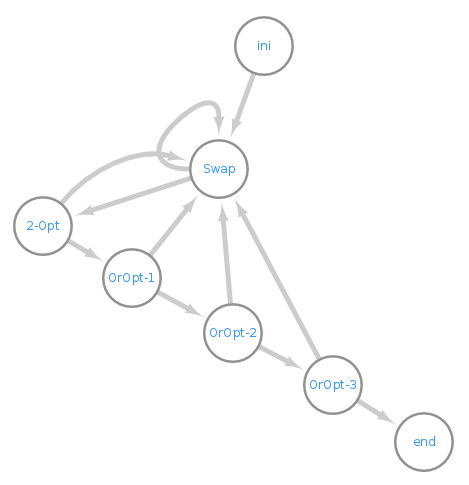
\includegraphics[scale=0.5]{figuras/rvnd/RVND_dataflow_nomes.png}}
    \caption{Arquitetura simplificada do dataflow para o RVND com as vizinhanças utilizadas.}
    \label{fig:rvndGraph}
\end{figure}

A implementação do nó operador (\textit{Swap, 2-Opt, OrOpt-1, OrOpt-2, OrOpt-3}) é tão simples quanto o Algoritmo~\ref{alg:rvndOper} e cada estratégia de vizinhança é atrelada a um nó operador, sendo que a ordem desses é variada para cada execução do método para caracterizar o RVND, a decisão de para qual nó enviar o resultado é tomada pela configuração do dataflow.
Quando a solução atinge o nó final (\textit{end}) esta é salva e o processo termina.

\begin{algorithm}[htpb]
\caption{Nó de vizinhança do RVND}
\label{alg:rvndOper}
\begin{algorithmic}[1]
    \Function{RVND\_Oper}{Solução: $s$}
        \Let{$s'$}{melhor solução de $N^k(s)$}
        \Let{$improvFlag$}{$f(s') < f(s)$}
        \Return{$(s', improvFlag)$}
    \EndFunction
\end{algorithmic}
\end{algorithm}

Pode ser visto destacado na Figura~\ref{fig:rvndGraphDestacado} uma vizinhança com suas ligações ao grafo dataflow, uma de entrada de dados e duas outras de saída que são para o caso de haver ou não uma melhoria no valor da solução.
Para acoplar uma nova vizinhança ao algoritmo basta que seja inserido um novo nó de enumeração com sua entrada de dados vindo do nó anterior e duas saídas de dados, uma retornando para a primeira vizinhança e outra para a vizinhança seguinte, conforme destacado na mesma figura.

\begin{figure}[htbp]
    \centerline{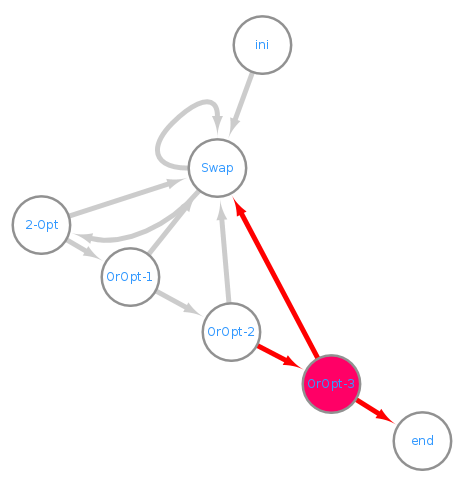
\includegraphics[scale=0.5]{figuras/rvnd/RVND_dataflow_nomesDestacado.png}}
    \caption{Uma vizinhança e suas ligações ao grafo dataflow no RVND.}
    \label{fig:rvndGraphDestacado}
\end{figure}

\subsubsection{Passo iterativo}

Utilizando o termo convencionado na seção~\ref{subsec:passoIterativo}, cada passo iterativo do RVND retorna a melhor solução encontrada para a vizinhança atual.
Assim sendo $N^k$ a vizinhança atual temos o passo iterativo para o RVND expresso na Equação~\ref{eq:rvndPassoIterativo}.
\begin{equation} \label{eq:rvndPassoIterativo}
    \rho^{RVND}(s) = s' \in N^k \quad \textrm{sendo} \quad f(s') < f(s''), \forall s'' \in N^k(s) \land s'' \ne s
\end{equation}
Fazendo uso da notação de movimentos temos podemos escrever \ref{eq:rvndPassoIterativo} como a Equação~\ref{eq:rvndPassoIterativoMovimento}.
\begin{equation} \label{eq:rvndPassoIterativoMovimento}
    \rho^{RVND}(s) = m \circ s \quad \textrm{com} \quad m \in M^k \land \widehat{m} < \widehat{m_i} \mid \forall m_i \in M^k
\end{equation}
